\begin{figure}[htbp]
\centering
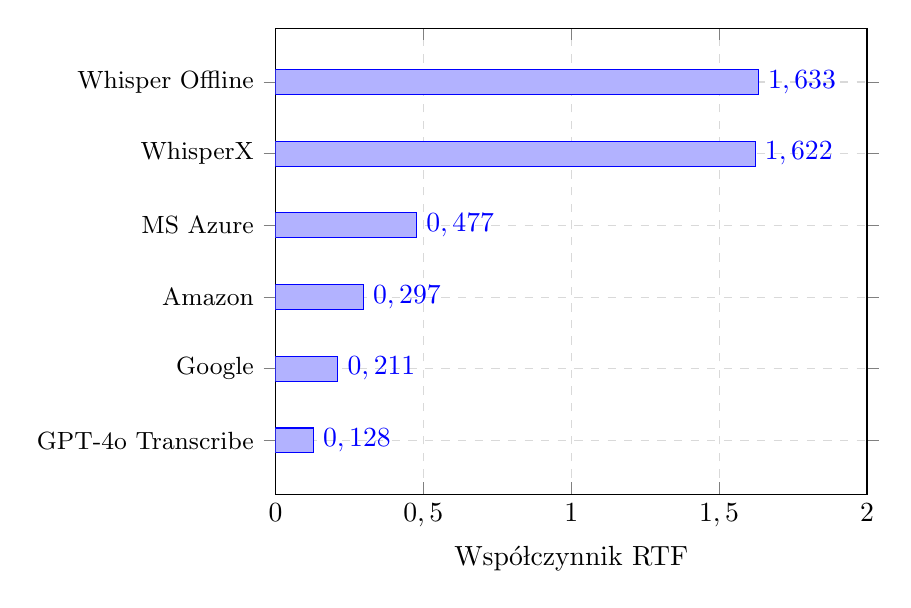
\begin{tikzpicture}
\begin{axis}[
    xbar,
    symbolic y coords={
        GPT-4o Transcribe,
        Google,
        Amazon,
        MS Azure,
        WhisperX,
        Whisper Offline
    },
    ytick=data,
    nodes near coords,
    nodes near coords align={horizontal},
    nodes near coords style={
        /pgf/number format/fixed,
        /pgf/number format/precision=3,
        /pgf/number format/fixed zerofill,
        /pgf/number format/dec sep={,},
    },
    xlabel={Współczynnik RTF},
    xmin=0, xmax=2.0,
    xtick={0,0.5,1.0,1.5,2.0},
    xticklabel={\pgfmathprintnumber[fixed,precision=1,dec sep={,}]{\tick}},
    bar width=9pt,
    enlarge y limits=0.15,
    y tick label style={font=\small},
    width=0.75\textwidth,
    height=7.5cm,
    grid=major,
    grid style={dashed, gray!30}
]
\addplot coordinates {
    (0.128,GPT-4o Transcribe)
    (0.211,Google)
    (0.297,Amazon)
    (0.477,MS Azure)
    (1.622,WhisperX)
    (1.633,Whisper Offline)
};
\end{axis}
\end{tikzpicture}
\caption{Porównanie współczynnika RTF dla badanych modeli ASR.}
\label{fig:rtf_comparison}
\end{figure}
